\section{Loggable\-End\-Line Class Reference}
\label{classLoggableEndLine}\index{LoggableEndLine@{LoggableEndLine}}
{\tt \#include $<$Loggable.hpp$>$}

Inheritance diagram for Loggable\-End\-Line::\begin{figure}[H]
\begin{center}
\leavevmode
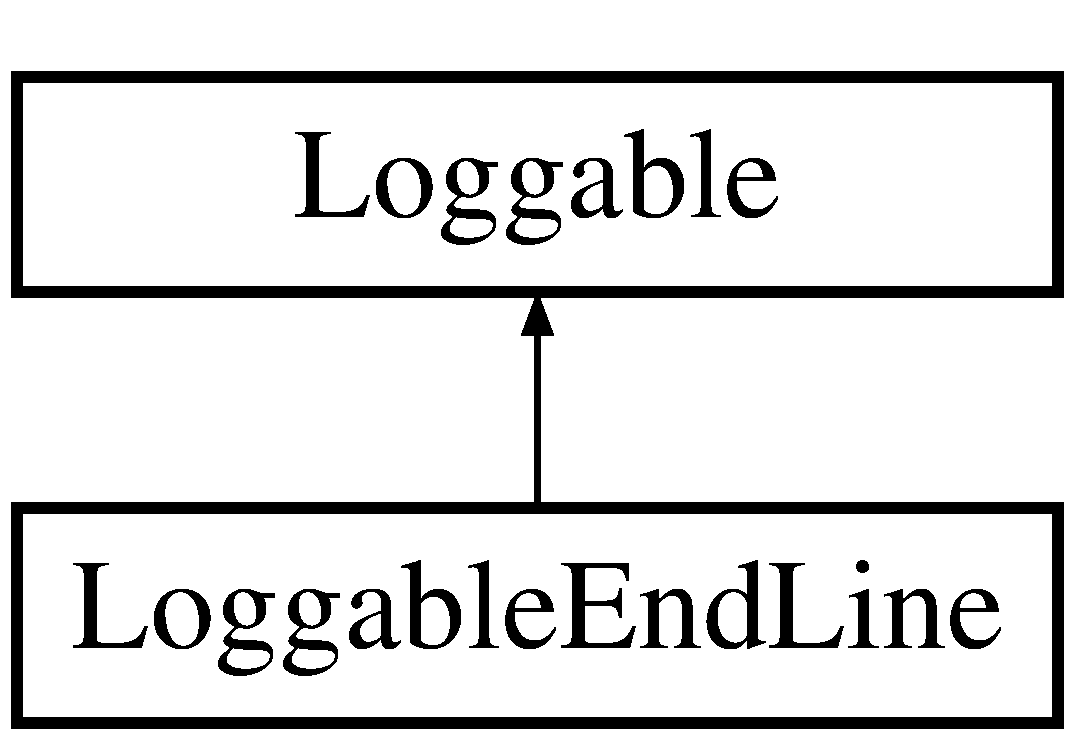
\includegraphics[height=2cm]{classLoggableEndLine}
\end{center}
\end{figure}
\subsection*{Public Member Functions}
\begin{CompactItemize}
\item 
virtual std::string {\bf to\-String} () const 
\end{CompactItemize}


\subsection{Detailed Description}
This predefined log token is a wrapper for the new line character.



\subsection{Member Function Documentation}
\index{LoggableEndLine@{Loggable\-End\-Line}!toString@{toString}}
\index{toString@{toString}!LoggableEndLine@{Loggable\-End\-Line}}
\subsubsection{\setlength{\rightskip}{0pt plus 5cm}virtual std::string Loggable\-End\-Line::to\-String () const\hspace{0.3cm}{\tt  [inline, virtual]}}\label{classLoggableEndLine_a0}


Clients should use this interface memeber to provide the logger with a formatted message.

Implements {\bf Loggable} {\rm (p.\,\pageref{classLoggable_a0})}.

The documentation for this class was generated from the following file:\begin{CompactItemize}
\item 
Loggable.hpp\end{CompactItemize}
